\section{Synthesis}
The tessellation phase extracts tiles $N\times N$ from each image. Starting from a matrix of grey pixels, represented as a matrix in $\left[0,1\right]^{h \times w}$, where $h$ is the height and $w$ the width of the image.

\noindent At the end of this procedure, each image is represented as a list of tiles, which is why this phase is called ‘synthesis’: in fact, it is difficult to reconstruct the original image from the tiles. This process considerably complicates any attempt to falsify the work, as manually reconstructing an image with a tessellation distribution similar to the original is extremely complicated. Furthermore, the size of the tiles in the representation is small, but large enough to capture small automatisms of the author's hand, details that are difficult to reproduce voluntarily.

\begin{algorithm}[ht]
\caption{Algorithm for tile extraction}
\begin{algorithmic}[1]
\Function{TilesExtraction}{$\textnormal{M}, \textnormal{h}, \textnormal{w}$}
    \State declare $v$ as matrix $N \times N$ \Comment{$N$ is size of tiles}
    \State $L \gets \texttt{empty list}$ \Comment{will have $(\textnormal{h} - N + 1)\times(\textnormal{w} - N+1)$ elements}
    \For{$row \gets 0$ to $\textnormal{h} - N$, $col \gets 0$ to $\textnormal{w} - N$}
        \For{$i \gets 1$ to $N$, $j \gets 1$ to $N$}
            \State $v[i][j] \gets \textnormal{M}[row + i][col + j]$
        \EndFor
        \State call \texttt{Append}($L$, $v$)
    \EndFor
\EndFunction
\label{alg:SequentialTilesExtraction}
\end{algorithmic}
\end{algorithm}

\begin{figure}[ht]
    \centering
    \begin{subfigure}{0.4\linewidth}
        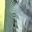
\includegraphics[width=\linewidth]{Figures/example_detail.png}
        \caption{Image detail $32 \times 32$.}
    \end{subfigure}
    \hspace{2cm}
    \begin{subfigure}{0.4\linewidth}
        
\includegraphics[width=\linewidth]{Figures/example_tiles.png}
        \caption{List of tiles $8 \times 8$.}
    \end{subfigure}
    \caption[Illustration of synthesis process]{The synthesis process convert an image in a list of its tiles.}
    \label{fig:puffer_tiles}
\end{figure}
